% !TEX TS-program = pdflatex
% !TEX encoding = UTF-8 Unicode

% This is a simple template for a LaTeX document using the "article" class.
% See "book", "report", "letter" for other types of document.

\documentclass[11pt]{article} % use larger type; default would be 10pt

\usepackage[utf8]{inputenc} % set input encoding (not needed with XeLaTeX)

%%% Examples of Article customizations
% These packages are optional, depending whether you want the features they provide.
% See the LaTeX Companion or other references for full information.

%%% PAGE DIMENSIONS
\usepackage{geometry} % to change the page dimensions
\geometry{a4paper} % or letterpaper (US) or a5paper or....
% \geometry{margin=2in} % for example, change the margins to 2 inches all round
% \geometry{landscape} % set up the page for landscape
%   read geometry.pdf for detailed page layout information

\usepackage{graphicx} % support the \includegraphics command and options

% \usepackage[parfill]{parskip} % Activate to begin paragraphs with an empty line rather than an indent

%%% PACKAGES
\usepackage[spanish]{babel}
\usepackage{booktabs} % for much better looking tables
\usepackage{array} % for better arrays (eg matrices) in maths
\usepackage{paralist} % very flexible & customisable lists (eg. enumerate/itemize, etc.)
\usepackage{verbatim} % adds environment for commenting out blocks of text & for better verbatim
\usepackage{subfig} % make it possible to include more than one captioned figure/table in a single float
% These packages are all incorporated in the memoir class to one degree or another...

%%% HEADERS & FOOTERS
\usepackage{fancyhdr} % This should be set AFTER setting up the page geometry
\pagestyle{fancy} % options: empty , plain , fancy
\renewcommand{\headrulewidth}{0pt} % customise the layout...
\lhead{}\chead{}\rhead{}
\lfoot{}\cfoot{\thepage}\rfoot{}

%%% SECTION TITLE APPEARANCE
\usepackage{sectsty}
\allsectionsfont{\sffamily\mdseries\upshape} % (See the fntguide.pdf for font help)
% (This matches ConTeXt defaults)

%%% ToC (table of contents) APPEARANCE
\usepackage[nottoc,notlof,notlot]{tocbibind} % Put the bibliography in the ToC
\usepackage[titles,subfigure]{tocloft} % Alter the style of the Table of Contents
\renewcommand{\cftsecfont}{\rmfamily\mdseries\upshape}
\renewcommand{\cftsecpagefont}{\rmfamily\mdseries\upshape} % No bold!

%%% END Article customizations

%%% The "real" document content comes below...

\title{Procesamiento de archivos  XML  en Python}
\author{Alvarado J.,Lasso H. \&  Lozano E.}
%\date{} % Activate to display a given date or no date (if empty),
         % otherwise the current date is printed 

\begin{document}
\maketitle

\section{Introducción}
El propósito de nuestro proyecto es que  mediante un analizador de texto en este caso el parseo comprobar si un archivo xml esta bien formado ,comprobar si el parseo es válido y poder realizar consultas sobre la información contenida en el archivo .\\ \\
El lenguaje de programación que utilizaremos es Python que cuenta con estructuras de datos eficientes y de alto
nivel y un enfoque simple pero efectivo a la programación orientada a objetos.\\ \\
La elegante sintaxis de Python y su tipado dinámico, junto con su naturaleza interpretada, hacen de éste un lenguaje ideal para scripting y desarrollo rápido de aplicaciones en diversas áreas y sobre la mayoría de las plataformas\\ \\
Python permite escribir programas compactos y legibles. Los programas en Python son típicamente más cortos que sus
programas equivalentes en C, C++ o Java por varios motivos:
\begin{itemize}
\item los tipos de datos de alto nivel permiten expresar operaciones complejas en una sola instrucción
\item la agrupación de instrucciones se hace por sangría en vez de llaves de apertura y cierre
\item  no es necesario declarar variables ni argumentos.
\end{itemize}
Estas son suficientes razones por las cuales Python es un lenguaje adecuado para hacer un parse de XML a una estructura manejable.

\section{Alcance}
Consiste en extraer la información que contiene un archivo xml, analizar su contenido , representarlo en una estructura y realizar funciones que nos permitan consultar su contenido.

\section{Descripción}
Se podría pensar en un documento XML como una estructura recursiva. Por tanto lo que buscamos es poder comprender en un solo vistazo las funcionalidades y/o módulos enteros. Con python pretendemos definir recursividad que implemente las estructuras anidadas del documento XML. Ya que en general, en cualquier XML se encuentran estructuras defininidas y etiquetadas. Es decir las definidas con los simbolos de mayor o menor: $<$f$>$abc$<$/f$>$. Que pueden ser en parejas  ( $<$f$>$ ,$<$/f$>$) o únicas (apertura y cierre) ($<$f ... /$>$). Y que recursivamente pueden contener más parejas de etiquetas o texto plano.
Nuestra decisión de programación fue leer el documento XML y su conjunto de datos, para representarlo como una Lista en Python. Pero no una Lista de Enteros o de Cadenas de Texto sino una Lista de un Tipo de Dato. \\ Haskell permite que definamos un Dato con sus características y a su vez el Tipo de Dato de las mismas. Por lo que definimos tres de estas en nuestro proyecto: Device, Group y Capability. Y al final lo que tuvimos como resultado fue una Lista que almacena Device.
\begin{itemize}
\item Lo que tenemos es una Lista de Devices que tiene como elementos  idD , useragent, actualdevice , fallback  y una lista de groups. Por medio del fallback del Device se hace uso de la orientación a objetos de Python y se tiene un puntero al Device que es fallback.
\item La lista de Group tiene  elementos  de tipo Group con las siguientes características : idG y  una lista de capabilities .
\item La lista de Capabilities tiene elementos de tipo Capability con estas características : name  y value .
\end {itemize}
\begin{center}
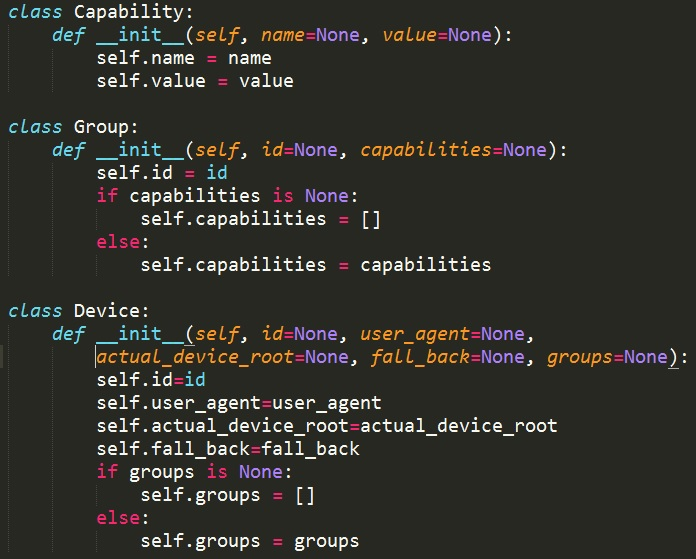
\includegraphics[scale=0.55]{Imagenes/1.jpg}
\\ Los tipos de datos construidos en Python
\end{center}

\section{¿Qué se implementó y qué no se implementó? }
\subsection{Lo implementado} 
Una vez extraída la información del archivo xml, la representamos en una lista de Devices que contiene elementos de tipo Device que se puede enlazar a su device fallback, contiene una lista de Groups que tienen elementos de tipo Group y cada Group contiene una lista  de  Capabilities que tienen elementos de tipo Capability.
\begin{center}
La lista creada en Python de Devices
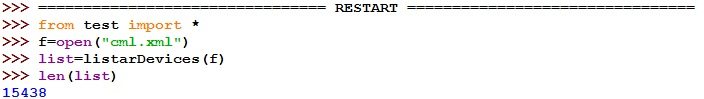
\includegraphics[scale=0.80]{Imagenes/3.jpg}
\\Un ejemplo de lo que hay en la lista obtenida, y sus respectivos valores
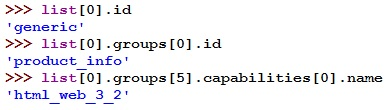
\includegraphics[scale=0.80]{Imagenes/4.jpg}
\end{center}
Con la lista de Devices ya obtenida podemos consultar la información de cada Device , Group o Capability. 
\begin{center}
Consultas en Python\\
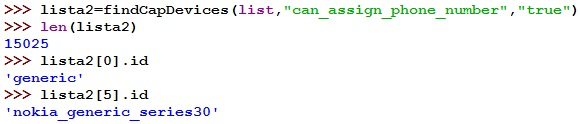
\includegraphics[scale=0.80]{Imagenes/5.jpg}
\end{center}
\subsection{Lo no implementado} 

\section{Observaciones}
\begin{itemize}
\item  Toda la sintaxis de Python esta basada en el correcto acomodo de espacios e indentación, lo cual se presta a confusiones. En este caso es recomendable encontrar un buen editor de texto que nos marque correctamente los espacios, o nos ayude con colores, figuras o marcas dependiendo del lenguaje en el que trabajemos. Aunque en este caso Python. El editor de texto usado fue Sublime Text 2
\begin{center}
Correcta indentación en Python con Sublime Text 2\\
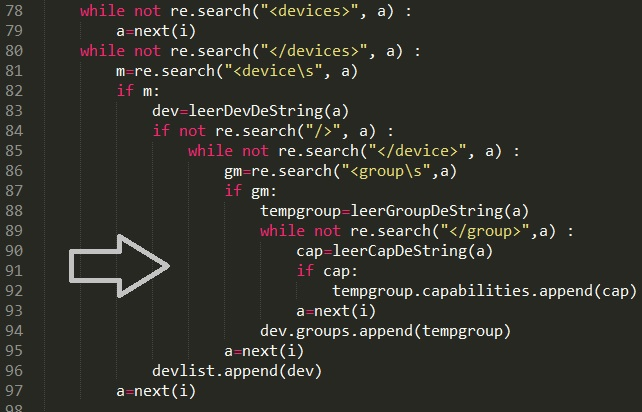
\includegraphics[scale=0.80]{Imagenes/6.jpg}
\end{center}
\item  Para leer el archivo XML, y hacer el respectivo linkeo al fallback de cada dispositivo tuvimos la necesidad de hacer una busqueda, y lo haciamos de manera lineal. En este caso fue necesario encontrar un algoritmo de Búsqueda eficiente, para mejorar el tiempo en el que se cargaba la lista de Devices en nuestra estructura.
\end{itemize}

\section{ Conclusiones}
\begin{itemize}
\item Python es un lenguaje muy cómodo y fácil de implementar. El hecho de que no se necesiten llaves, ni corchetes para las funciones, que no se definan los tipos de datos de las variables, y que se puedan crear de forma muy sencilla; hace a Python un lenguaje muy versátil y elegible como favorito a la hora de programar.
\item Python permite separar nuestro programa en módulos que pueden reusarse en otros programas en Python.
\item En cualquier búsqueda que realizemos es muy importante analizar el algoritmos que usemos, no es necesario que nosotros creemos uno. Lo importante es saber que existen ya implementados y que están disponibles para nuestro uso. Siempre en busca de una programación eficiente.
\end {itemize}



\end{document}
